% !TEX program = lualatex
\documentclass[11pt]{article}

% -------- LuaLaTeX : polices et langue --------
\usepackage{fontspec}
\setmainfont{Latin Modern Roman}
\setsansfont{Tex Gyre Heros}
%\renewcommand{\familydefault}{\sfdefault} % force le sans serif par défaut
\usepackage{polyglossia}
\setdefaultlanguage{french}

% -------- Mise en page --------
\usepackage[a4paper,margin=1cm]{geometry}
\usepackage{multicol}
\usepackage{fancyhdr}
\pagestyle{empty}
\usepackage[most]{tcolorbox}
\usepackage{graphicx}

% -------- Mathématiques --------
\usepackage{amsmath,amssymb,mathtools}
\usepackage{icomma}
% \sisetup{locale=FR}

\usepackage{enumitem}
\setlist[itemize]{left=0pt}
\setlist[enumerate]{left=0pt, label=\textbf{\arabic*}.}

\usepackage{ProfCollege}
\usepackage{ProfMaquette}

\usepackage{tabularray}

% -------- Divers --------
\setlength{\parindent}{0pt}

\begin{document}

\begin{Maquette}[Fiche]{Theme=Agrandissement et réduction, Niveau=Troisième}

   \begin{exercice}
      Tom a inséré une image dans un fichier de traitement de texte. L’image étant trop petite, il l’a donc agrandie. Quelle est à présent la hauteur de l’image ?
      \begin{center}
         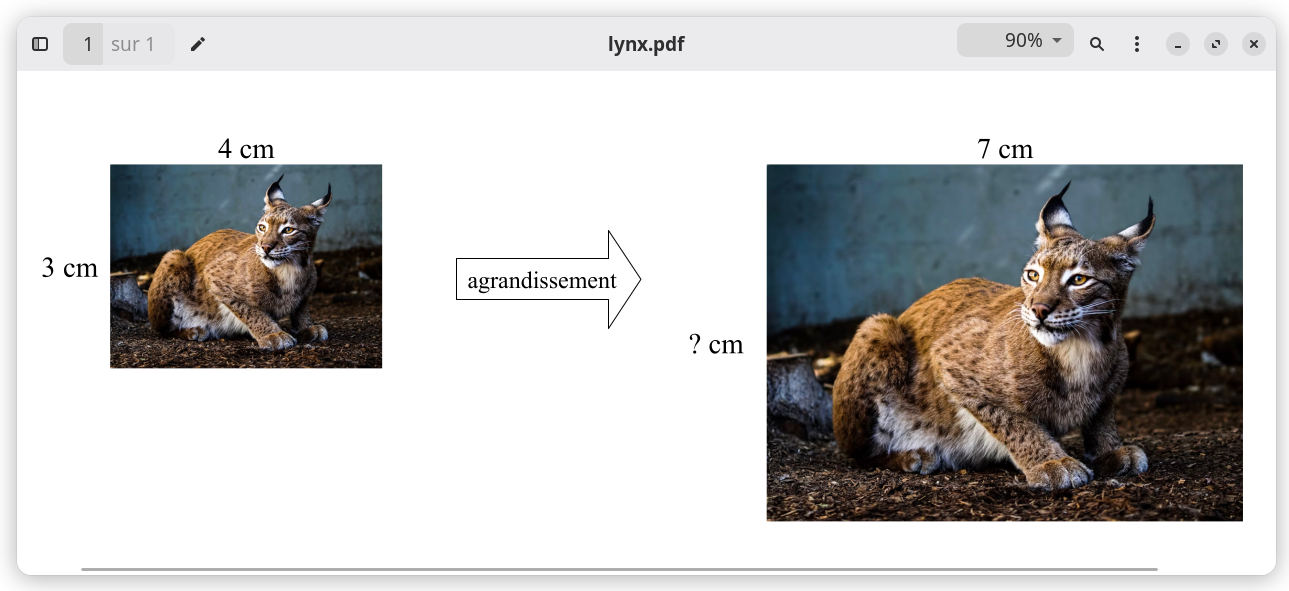
\includegraphics[width=.9\linewidth]{Images/Exercice1-Lynx.png}
      \end{center}
   \end{exercice}

   \begin{multicols}{2}

      \begin{exercice}
         \begin{enumerate}
            \item Léo pense que pour que deux figures soient dans une situation d’agrandissement/réduction, il suffit qu’elles aient les mêmes angles. Démontre que cela est faux en proposant un \emph{contre-exemple} à l’aide de deux quadrilatères.
            \item Anna pense qu’il suffit qu’elles aient des longueurs proportionnelles. Démontre que cela est également faux.
         \end{enumerate}

      \end{exercice}

      \begin{exercice}
         On agrandit un triangle rectangle :
         \begin{center}
            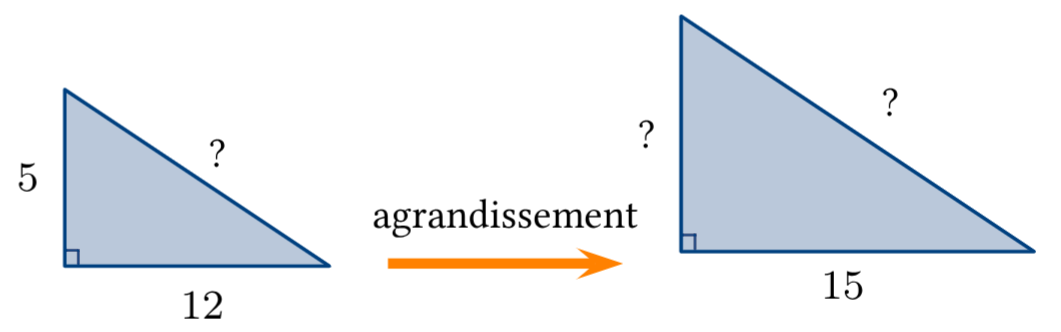
\includegraphics[width=.9\linewidth]{Images/Exercice3.png}
         \end{center}
         \begin{enumerate}
            \item Quel est le rapport d’agrandissement ?
            \item Calcule les longueurs manquantes.
         \end{enumerate}
      \end{exercice}
   \end{multicols}
   \newpage

   \begin{multicols}{2}
      \begin{exercice}
         Dans chaque situation :
         \begin{itemize}
            \item indique comment on passe de la $\textrm{Figure}_1$ à la $\textrm{Figrue}_2$ : agrandissement ou réduction
            \item calcule le rapport d’agrandissement ou de réduction
            \item calcule les longueurs manquantes sur les deux figures
         \end{itemize}

         \textbf{Situation 1}
         \begin{center}
            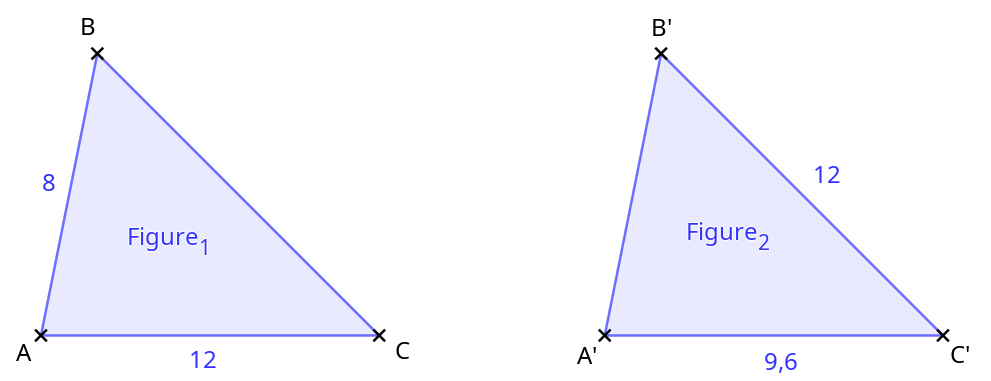
\includegraphics[width=\linewidth]{Images/ex4-2.png}
         \end{center}

         \textbf{Situation 2}
         \begin{center}
            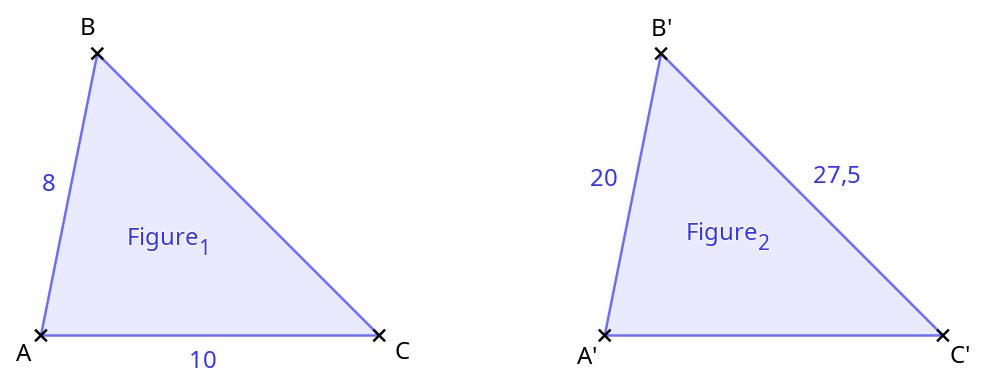
\includegraphics[width=\linewidth]{Images/ex4-1.png}
         \end{center}

         \textbf{Situation 3}
         \begin{center}
            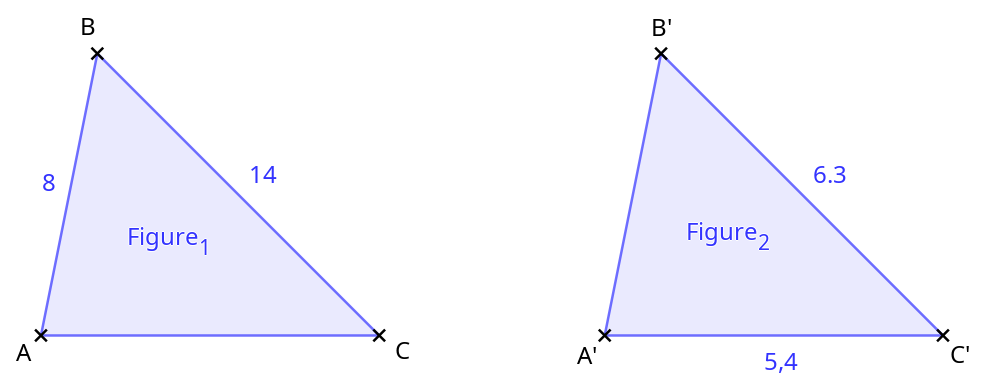
\includegraphics[width=\linewidth]{Images/ex4-3.png}
         \end{center}
      \end{exercice}
      \columnbreak
      \begin{exercice}
         \begin{enumerate}
            \item Trace un rectangle $\textrm{ABCD}$ tel que $\textrm{AB} = \Lg{3}$ et $\textrm{BC} = \Lg{2}$.
            \item Trace $\textrm{A’B’C’D’}$ qui est un agrandissement de $\textrm{ABCD}$ de rapport $3$.
            \item Quel est le périmètre de $\textrm{ABCD}$ ?
            \item[] Et celui de $\textrm{A’B’C’D’}$ ?
            \item Quelle est l’aire de $\textrm{ABCD}$ ?
            \item[] Et celle de $\textrm{A’B’C’D’}$ ?
         \end{enumerate}
      \end{exercice}
      
      \begin{exercice}
         Un architecte a réalisé une maquette d’une maison à l’échelle $1:50$.
         \begin{enumerate}
            \item Quel est le rappport d’agrandissement qui permet de passer de la maquette à la maison réelle ?
            \item La hauteur du toit sur la maquette est de \Lg{12}. Quelle est, en mètres, la hauteur réelle du toit ?
            \item La surface du salon sur la maquette est de \Aire[dm]{80}. Quelle est, en $\textrm{m}^2$, la surface réelle du salon ?
            \item Le volume du garage sur la maquette est de \Vol[cm]{576}. Quel est, en $\textrm{m}^3$, son volume réel ?
         \end{enumerate}

      \end{exercice}
   \end{multicols}
   \newpage
   \begin{exercice}
      \begin{center}
         \fbox{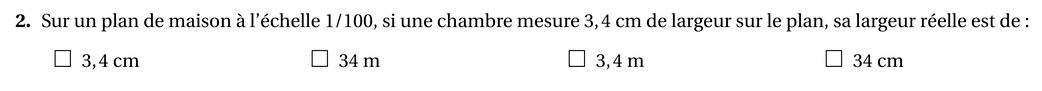
\includegraphics[width=\linewidth]{Images/ex7-2.png}}
         
         \vspace{.3cm}
         \fbox{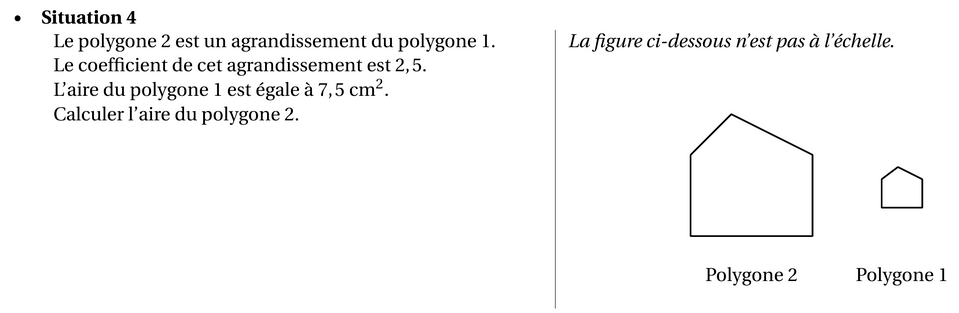
\includegraphics[width=\linewidth]{Images/ex7-1.png}}
         
         \vspace{.3cm}
         \fbox{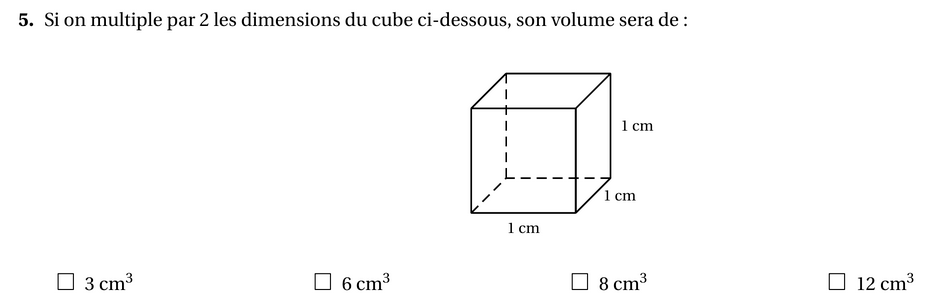
\includegraphics[width=\linewidth]{Images/ex7-3.png}}
      \end{center}
   \end{exercice}
   \newpage
   \begin{exercice}
      \begin{center}
         \fbox{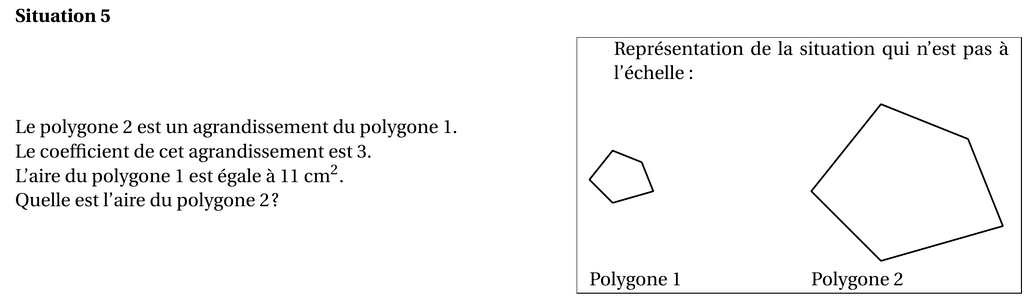
\includegraphics[width=\linewidth]{Images/ex7-4.png}}

         \vspace{.3cm}
         \fbox{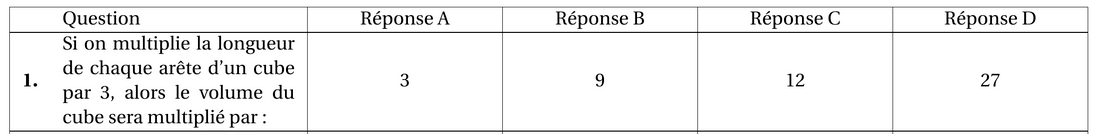
\includegraphics[width=\linewidth]{Images/ex7-6.png}}
         
         \vspace{.3cm}
         \fbox{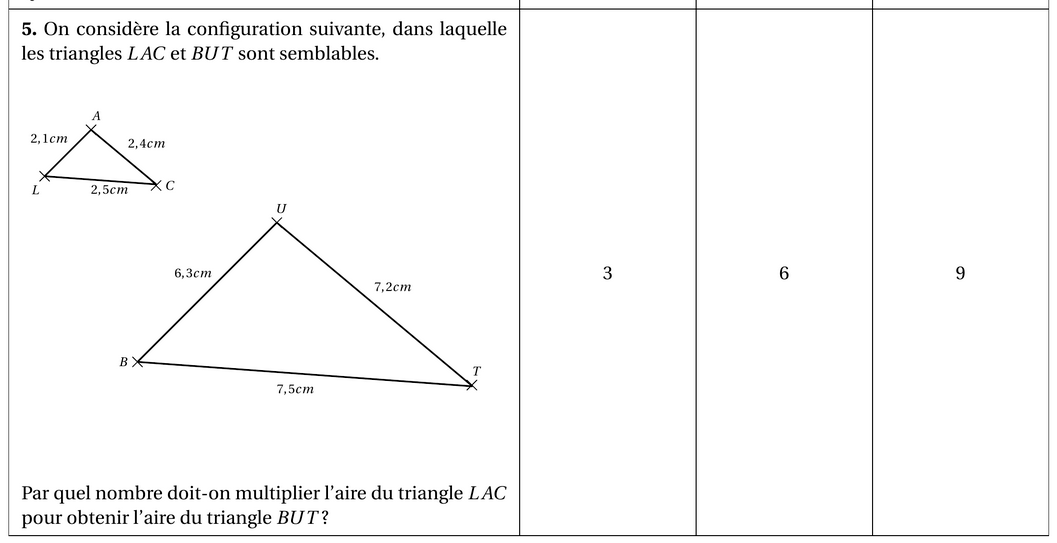
\includegraphics[width=\linewidth]{Images/ex7-5.png}}

      \end{center}
   \end{exercice}
\end{Maquette}

\end{document}
